\chapter{Literature review}
\section{General Introduction to Ferromagnetics}

\subsection{Origin of Ferromagnetism}
In all materials, the atomic masses are from the atomic nucleus, while the electrical, chemical and magnetic properties are determined by the electronic structure. Electrons are distributed in specific shells at definite distances from the nucleus, which is due to the different energy level in each shell. In the FM elements, including $\alpha$-Fe, Co, Ni and Gd, there are three important features:

\begin{enumerate}
\item There must be an unfilled inner electron shell within the atom.
\item There must be uncompensated electronic spins in the unfilled inner shell.
\item The atoms must form a crystal lattice having a lattice constant at least 3
times the radius of the unfilled electron shell.
\end{enumerate}

Electrons have an intrinsic property called spin that contributes to their magnetic moment. The classical model of electron spin is the electron spinning on its
axis, i.e. either spin-up or spin-down. Macroscopic magnetic properties of materials are a consequence of magnetic moments associated with individual electrons, which is the sum of spin moment Figure~\ref{fig:electron}a and orbital moment Figure~\ref{fig:electron}b.

\begin{figure}[H]
\centering
\captionsetup{justification=centering,margin=2cm}
	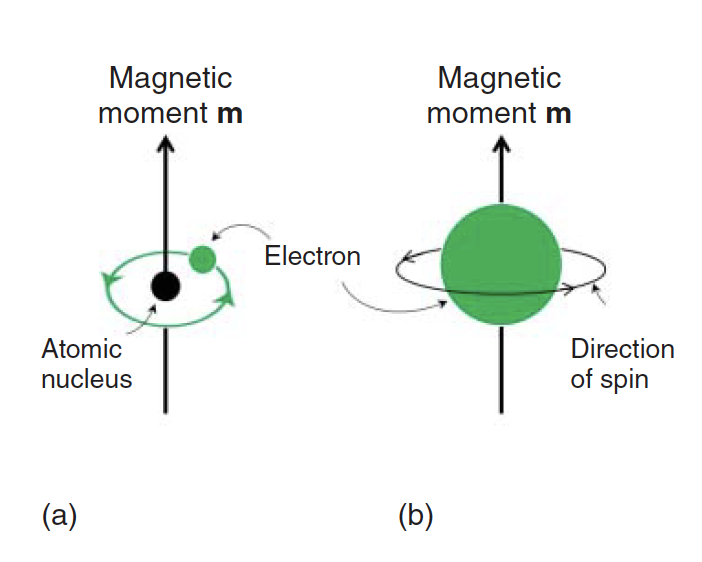
\includegraphics{fig/review/electron.png}
	\caption[Diagram showing the magnetic moment associated with orbital and spin motion of an electron.]{Diagram showing the magnetic moment associated with (a) orbital motion and (b)spin motion of an electron.}
\label{fig:electron}
\end{figure}

The magnetic susceptibility $\chi$ is a dimensionless proportionality
constant that indicates the degree of magnetization of a material in response to an applied magnetic field, and is given by:
\begin{equation}
\chi = \frac{M}{H}
\end{equation}
where $\chi$ is the magnetic susceptibility, $M$ is the magnetization of the material, and $H$ is the applied field.

Depending on the magnetic ordering and the sign, magnitude and
temperature dependence of the magnetic susceptibility, the magnetic materials are classified into diamagnetic, paramagnetic, ferromagnetic (FM), antiferromagnetic (AFM) and ferrimagnetic (FiM) materials.

\subsection{T-symmetry}
Generally T-symmetry or Time Reversal symmetry is the symmetry of physical laws under a time reversal transformation $( \tau )$.
\begin{equation}
\tau : t \rightarrow -t
\end{equation}

The origin of ferromagnetism (FM) is time reversal symmetry breaking due to the existence of unpaired spin of electrons and the associated current \cite{eerenstein2006multiferroic}. 
This statement
can be understood by considering that if time is reversed, the spin or current
flow direction will thus be reversed and this results in magnetization direction
reversion, i.e. time reversal symmetry breaking.

\begin{equation}
\tau : \mu = - \mu
\end{equation}

In other words as it is illustrated on Figure \ref{fig:time_reverse} the local magnetic moment \textbf{m} may be represented classically by a charge that dynamically traces an orbit, as indicated by the arrowheads. A spatial inversion produces no change, but time reversal switches the orbit and thus \textbf{m}.

\begin{figure}[H]
	\centering
	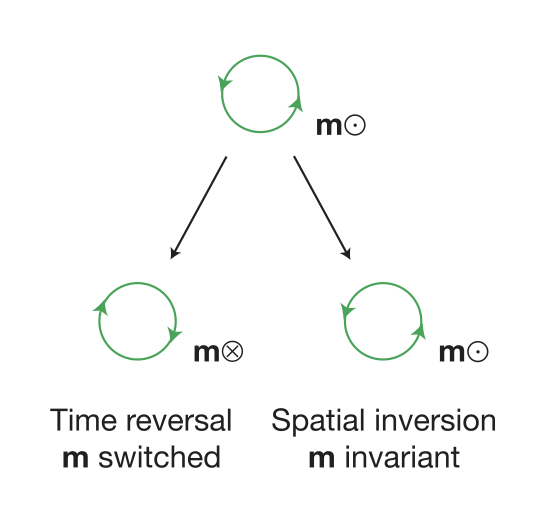
\includegraphics{fig/review/time_reverse.png}
	\caption[Illustration of time reversion symmetry breaking]{Illustration of time reversion symmetry breaking \cite{eerenstein2006multiferroic}}
\label{fig:time_reverse}
\end{figure}

Thus, magnetic ordering always breaks at least one symmetry of the crystal, the invariance under time inversion. Invariance under rotations around axes not coinciding with the ordered moments also disappears. This symmetry braking is not related to asymmetries in the spin Hamiltonian.
Spin Hamiltonians are constructed to describe the behaviour of the degrees of freedom of atoms or ions occupying lattice sites.
Therefore, they have the full symmetry of the lattice.
For instance, in a cubic lattice the bilinear term describing the interaction between magnetic moments can be written in the Heisenberg form:
\begin{equation}
H = -\frac{J_{ex}}{2}\sum \limits_{i, k} \left( S^{(i)}_x S^{(j)}_x + S^{(i)}_y S^{(j)}_y + S^{(i)}_z S^{(j)}_z \right)
\end{equation}

Here only nearest-neighbour interaction is included. Nearest neighbours are equivalent in a cubic lattice, hence the unique exchange parameter $J_{ex}$. In a tetragonal lattice, $z$ is not equivalent with $x$ and $y$ , the interaction Hamiltonian will include two exchange parameters and have the form:
\begin{equation}
H = -\frac{J_{ex}}{2}\sum \limits_{i, k}  \left[ J_ex \left( S^{(i)}_x S^{(j)}_x + S^{(i)}_y S^{(j)}_y \right) +J' S^{(i)}_z S^{(j)}_z \right]
\end{equation}

Evidently, anisotropic exchange is allowed. Disregarding single-ion magneto crystalline anisotropy, if , $J'/J>1$ the latter Hamiltonian describes a magnet with easy-axis anisotropy, if , $J'/J < 1$ with easy-plane anisotropy. 
In the case of extreme anisotropy we find the Hamiltonians which define two important models:

\begin{equation}
H_{Ising} = -\frac{J_{ex}}{2}\sum \limits_{i, k} S^{(i)}_z S^{(j)}_z 
\end{equation}

\begin{equation}
H_{XY} = -\frac{J_{ex}}{2}\sum \limits_{i, k} \left( S^{(i)}_x S^{(j)}_x + S^{(i)}_y S^{(j)}_y \right)
\end{equation}

As the Ising and XY models exclude some components of the spin vectors, the entities they describe can be looked upon as one- and two-dimensional moments, respectively.
However, this does not automatically make them low-dimensional models. The dimensionality is determined by the meaning of the indices $i$ and $j$. Those indicate sites in a lattice of well defined dimension.
Thus one can study three-dimensional Ising models or one-dimensional XY models; there is no contradiction in terms here.




\subsection{Types of magnetism}\label{sec:ordering}
In terms of magnetization, materials can be classified into paramagnetic, diamagnetic, ferrimagnetic (FiM), ferromagnetic (FM) and antiferromagnetic (AFM) as it is shown in Figure \ref{fig:magneticorder}.

\begin{figure}[H]
	\centering
	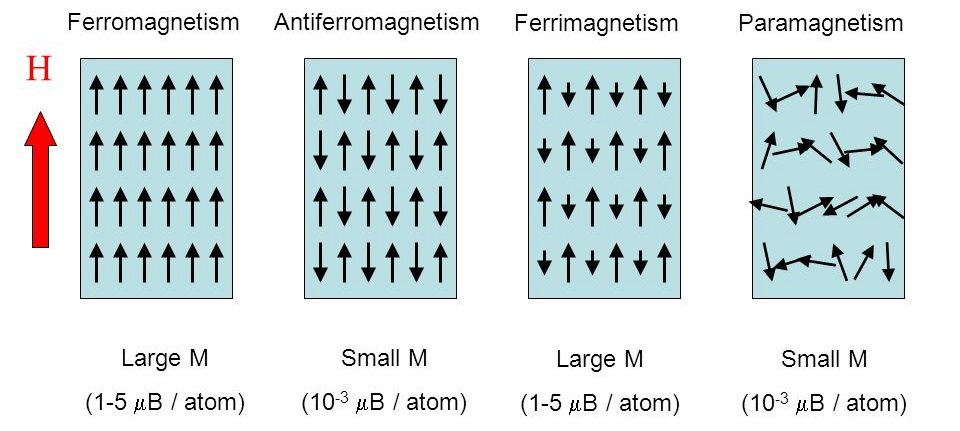
\includegraphics[width=130mm]{fig/review/magneticorder.png}
	\caption[Schematic illustration of various types of magnetism.]{Schematic illustration of various types of magnetism.}
\label{fig:magneticorder}
\end{figure}

A FM material usually forms permanent magnet or is attracted to magnets, and it undergoes phase change to paramagnetic above Curie temperature $(T_C)$ through a second-order phase transition.
FM (including FiM) is the strongest type; it is the only type that creates forces strong enough to be felt and is responsible for the common phenomena of magnetism encountered in everyday life.
An AFM has magnetization microscopically but has no macroscopic magnetization due to the cancelation of antiparallel spins of alternative layers. 
The temperature from an AFM to paramagnetic phase transition is called Néel temperature. FiM is a relatively weak FM, such as \ce{CoFe_2O_4} spinel. A diamagnetic generates weak but negative magnetization when a magnetic field is applied. 

Figure \ref{fig:table2} houses characteristic types of magnetization of pure elements in a solid-state and low temperature.

\begin{figure}[H]
	\centering
	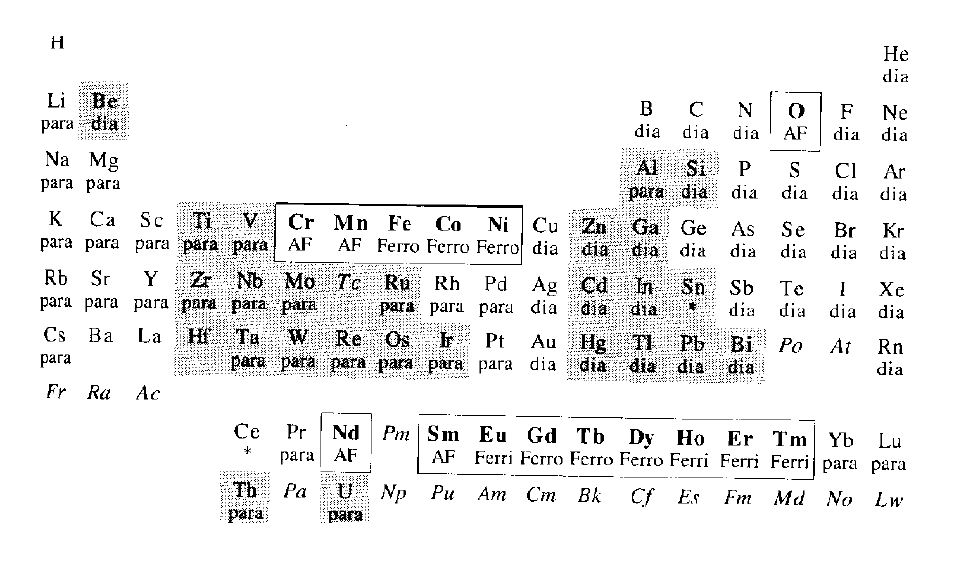
\includegraphics[width=100mm]{fig/review/tabel2.png}
	\caption[Magnetic properties of pure elements]{The magnetic properties of pure elements in a solid state at low temperature.}
	\label{fig:table2}
\end{figure}




A magnetic solid, made up of atoms with magnetic moment, has quantum exchange interactions that tend to align the magnetic moments at low temperature. When $T <T_C$, the macroscopic magnetization arises and retains even in the absence of a magnetic field. The magnetic moments tend to align in the same direction without the aid of an external magnetic field.
This is known as the FM phase. In the FM category, materials are divided into strong and weak ferromagnets.
By introducing the total particle number $N=N\uparrow+N\downarrow$ and the spin polarization $s=N\uparrow-N\downarrow$, a strong ferromagnet has almost $s = 100\%$ at the Fermi energy as shown in Figure~\ref{fig:dos}a, while a weak ferromagnet gets a smaller spin polarization and paramagnet has no net spin polarization Figure~\ref{fig:dos}  (b, c).

\begin{figure}[H]
\centering
\captionsetup{justification=centering,margin=2cm}
	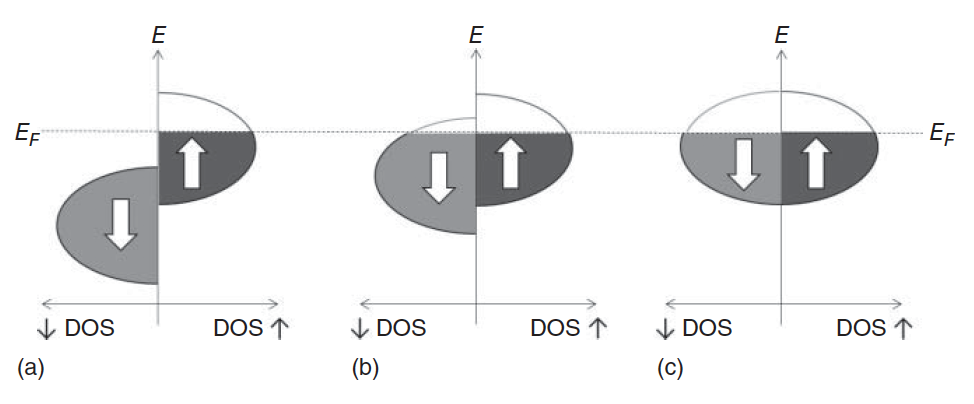
\includegraphics[width=130mm]{fig/review/dos.png}
	\caption[Schematic densities of states (DOSs) for ferromagnetism.]{Schematic densities of states (DOSs) for ferromagnetism: (a) strong ferromagnet, (b) weak ferromagnet, and (c) paramagnet.}
\label{fig:dos}
\end{figure}

Meanwhile, there is another type of magnets that possess magnetization
microscopically, but have no macroscopic magnetization due to the cancelation
of antiparallel spins of neighboring pairs – this is known as AFM phase.
A magnet that exhibits no macroscopic magnetization at high temperature (when $H = 0$) is known as the paramagnetic phase, in which the magnetic moment induced by the applied H-field is rather weak.
 Figure~\ref{fig:temp_mag} shows the relationship
between magnetization and temperature of a ferromagnet, where one can see
that the magnetization starts decreasing close to $T_C$, and when $T >T_C$, magnetic
moments align randomly resulting in zero macroscopic magnetization.
\begin{figure}[H]
	\centering
	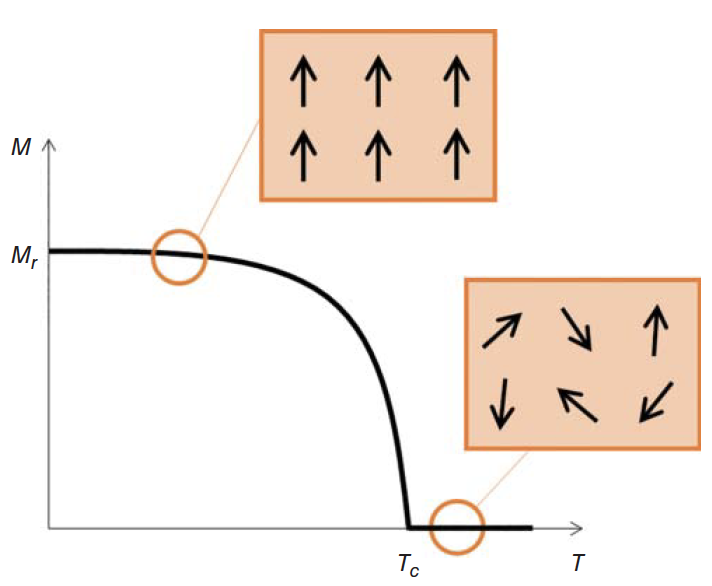
\includegraphics{fig/review/temp_mag.png}
	\caption[Illustration of magnetization versus temperature.]{Illustration of magnetization versus temperature.}
\label{fig:temp_mag}
\end{figure}

Any atoms or ions with existing unpaired electrons exhibit ferromagnetism
such as Fe, Co, and Ni. Magnetization can exist, even very weak, in
non-FM materials such as graphene as long as their defects or edge
structures induce dangling bonds with unpaired electrons \cite{Ma:2012aa, Liu:2013aa}. However, those FM materials with practical application
potentials are usually compounds containing Fe, Co, or Ni.


\section{Domain and Domain Walls}
In FM, materials, exchange, and dipolar couplings are competing.
The equality between both interactions leads to a state in which the local macroscopic magnetization is extremely small. Still, an almost parallel alignment of the moments is preserved at short distances.
In the absence of magnetocrystalline anisotropy, a gradual rotation of the moments takes place.
Overall, the material splits into a number of isolated zones, called magnetic domains.
Within each domain, the moments are parallel as required by coupling, the magnetization is directed along a precise so-called easy direction, as required by anisotropy. From one zone to another, the direction of magnetization changes so that the total magnetization disappears.
Between two neighboring domains, a gradual rotation of the moments takes place which defines a Bloch wall. A Bloch wall has a special parameter characteristic thickness, $\delta$, for which its value of energy per unit area, $\gamma$, is minimum. $\delta$ and $\gamma$ are given by :
\begin{align}
\delta = \pi \sqrt{A/K} \\
\gamma = 4 \sqrt{AK}
\end{align}

here $A$, the exchange constant expressed in $J/m$, characterises the strength of the exchange coupling and $K$ is the anisotropy constant expressed in $J/m^3$.
Most typically $\delta$ varies from 50 nm
in the $3d$ metals to 3 nm in high-anisotropy compounds (\ce{SmCo5}, \ce{Nd_2Fe_{14}B}).

\begin{table}[H]
\caption[Domain wall thickness]{Domain wall thickness}
\centering

\begin{tabular}{|l|c|}

\hline 
Magnetic material & Domain wall width (nm) \\ 
\hline 
Co & 14 \\ 
\ce{Nd_2Fe_{14}B} & 3.9 \\ 
\ce{Sm_2Fe_{17}N_3} & 3.6 \\ 
\ce{Sm_2Co_{17}} & 8.6 \\ 
FePd & 11.4 \\ 
\hline 
\end{tabular} 

\end{table}

In the general case, splitting of a FM material into domains separated by walls occurs spontaneously.
In a homogeneous material, the wall energy does not depend on the wall position.
 Under an applied external field $H$, the initial magnetization variation is to minimize the Zeeman energy and the dipolar energy. In a system of cubic symmetry, the susceptibility is equal to the inverse of the demagnetizing field slope; it is defined by the sample shape and not connected to the intrinsic material properties.
During this process, the magnetization variation occurs by growing the domains aligned by the applied field at the expense of others. The material is in the single domain state at a larger field, and magnetization variation occurs by moment rotation.


FM materials also exhibit domain structure where each domain has its own magnetization direction that can be switched by external magnetic field.
There are easy axes in FM materials that are the directions magnetic
moments should follow. For example, for a cubic structured FM material such as
Fe, the $\langle 100 \rangle$ directions are usually the easy axes, while for a hexagonal-structured FM material such as Co, the $\langle 0001\rangle$ are the easy axes. Due to this difference, in a cubic structure, both $90 ^\circ$ and $180^\circ$ magnetic domains can be formed (Figure~\ref{fig:domain_structure}a), while in a hexagonal structured FM material, the domains are usually aligned with an angle of $180 ^\circ $ (Figure~\ref{fig:domain_structure}b).

\begin{figure}[H]
\centering
\captionsetup{justification=centering,margin=2cm}
	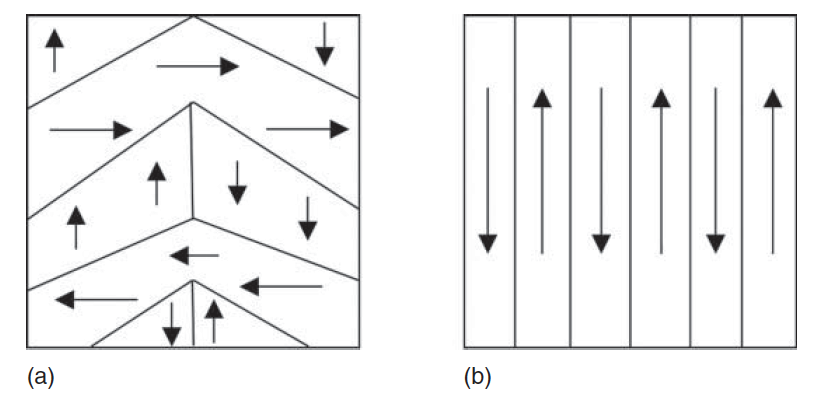
\includegraphics[width=110mm]{fig/review/domain_structure.png}
	\caption[Domain structures in cubic and FM materials.]{Domain structures in cubic (a) and hexagonal (b) structured FM materials.}
\label{fig:domain_structure}
\end{figure}

The easy axes of cubic-structured Ni are $\langle 111 \rangle$, so it can form $180 ^\circ$, $71 ^\circ$, and $109 ^\circ$ magnetic domains; these are possible angles between all $\langle 111 \rangle$ easy axes. The magnetization switching can be realized by not only external magnetic field but also mechanical stress.

FM domain wall is only one to a few atomic layers. Figure~\ref{fig:wall_structure}a illustrates the $180  ^\circ$ domain wall structure in FM materials, where the more common one is the Bloch wall, but in thinner films a Néel wall is often favored Figure \ref{fig:wall_structure}b. By contrast, Figure \ref{fig:wall_structure}c demonstrates a narrow domain wall (Ising type) structure usually as the case of a ferroelectric domain structure.

\begin{figure}[H]
\centering
\captionsetup{justification=centering,margin=2cm}
	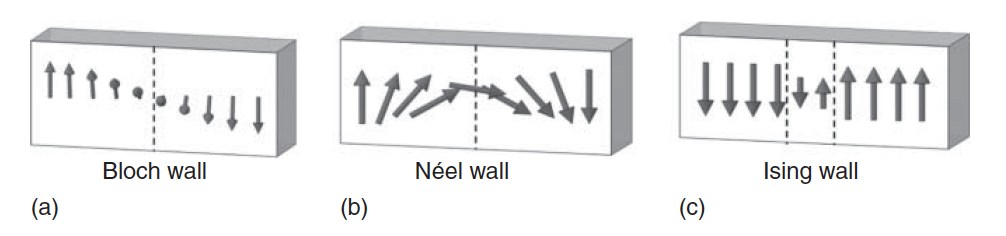
\includegraphics[width=150mm]{fig/review/wall_structure.png}
	\caption[Domain wall structures.]{Domain wall structures of (a) Bloch-type FM domain walls, (b) Néel-type FM domain walls, and (c) Ising-type ferroelectric domain walls.}
\label{fig:wall_structure}
\end{figure}

\subsection{Magnetic anisotropy}
Magnetic anisotropy is defined as the directional dependence of the magnetic
properties for materials. Specifically, the preferential direction for its magnetic moment in the absence of an applied magnetic field. Strong easy-axis anisotropy is a prerequisite for hard magnetism, while near-zero anisotropy is desirable for soft magnets.
Generally, the tendency for magnetization to lie along an easy axis is represented by the energy
density term:
\begin{equation}
E_a = K_1 \sin^2 \theta
\end{equation}

where $\theta$ is the angle between the magnetic field and the anisotropy axis, and $K_1$ is the
anisotropy constant, which ranges from $~1 kJ/m^3$ to more than $20 MJ/m^3$.  There are
several sources of magnetic anisotropy:
\begin{itemize}
\item Magnetocrystalline anisotropy: intrinsic property due mainly to spin-orbit coupling;
\item Shape anisotropy: induced by the nonspherical shape of the grains; 
\item Stress anisotropy: created by applied mechanical stress due to the existence of magnetostriction, which could alter the domain structure;
\item Exchange anisotropy: occurs when the interaction between antiferromagnet and a ferromagnet occurs at their interface;
\item Anisotropy induced by grain alignment and stress through magnetic
annealing, irradiation, and plastic deformation:
\begin{itemize}
\item Magnetic annealing: thermomagnetic treatment (heat treatment in a magnetic field) could introduce anisotropy in certain alloys;
\item Irradiation: when the materials are irradiated by neutron at high temperature in a magnetic field, the direction irradiated will become an
easy axis;
\item Plastic deformation: plastic tension/compression would cause the specimen volume in tension/compression parallel to the deformation axis, which is the preferred axis to magnetize.
\end{itemize}

\end{itemize}

\subsection{Magnetocrystalline anisotropy}
The magnetocrystalline anisotropy primarily arises from spin-orbit coupling.
When an external field tries to reorient the spin of an electron, the orbit of that electron
also tends to be reoriented. But the orbit is strongly coupled to the lattice and therefore
resists the attempt to rotate the spin axis. The energy required to rotate the spin system of
a domain away from the easy direction, anisotropy energy, is the energy required to
overcome the spin-orbit coupling. The strength of the magnetocrystalline anisotropy in
any particular crystal is measured by the magnitude of the anisotropy constant $K_1$, $K_2$, etc.
$L1_0$ structure in this research is in tetragonal symmetry, conventional expression for the
anisotropy energy in tetragonal symmetry is:
\begin{equation}
E_a = K_1 \sin^2 \theta + K_2 \sin^4 \theta + K'_2 \sin^4  \theta \cos 4\varphi + K_3 \sin^6 \theta +K'_3 \sin^6 \theta \sin 6 \varphi
\end{equation}

where $K_i$ are the anisotropy constants, $\theta$
is the angle between the magnetic field and the anisotropy axis, $\varphi$ is the angle between
the magnetization and the field.
The magnitude of the magnetocrystalline anisotropy generally decreases with
temperature more rapidly than the magnetization vanishes at the Curie temperature. Since
the anisotropy contributes strongly to the coercive field, it has a great influence on
industrial uses of FM materials. Materials with high magnetic anisotropy
usually have high coercivity; that is they are hard to demagnetize.
The high anisotropy of rare earth metals is mainly responsible for the strength of rare earth magnets, which are widely used in permanent magnets.

\section{Heisenberg spin model}
\label{section: Heisenberg spin model}

Magnetic systems are fundamentally quantum mechanical by nature therefore the exchange interaction - one of the most important properties of such systems also is a purely quantum mechanical effect. In addition to the properties at the electronic level, the properties of magnetic materials are heavily influenced by thermal effects which are typically difficult to incorporate into standard density functional theory (DFT) approaches. Therefore, models of magnetic materials should combine quantum mechanical properties with accurate thermodynamic theories. The simplest model of magnetism using this approach is the Ising model, which allows the atomic moments one of two allowed states along a fixed axis. The Ising model is quite useful as a descriptive system, but due to a large amount of approximation, the applicability of this model in relation to real materials is limited.
The more accurate theory is the Heisenberg spin model which describes the essential physics of magnetic material at the atomic level, where the energetics of a system of interacting atomic moments is given by a spin Hamiltonian. The spin Hamiltonian  typically has the form:

\begin{equation}
{\cal H}={\cal H}_{exc}+{\cal H}_{ani}+{\cal H}_{app}
\end{equation}

denoting terms for the exchange interaction $({\cal H}_{exc})$, magnetic anisotropy $({\cal H}_{exc})$, and externally applied magnetic fields $({\cal H}_{app})$ respectively. The dominant term in the spin Hamiltonian is the Heisenberg exchange energy, which arises due to the symmetry of the electron wavefunction and the Pauli exclusion principle which governs the orientation of electronic spins in overlapping electron orbitals. Due to its electrostatic origin, the associated energies of the exchange interaction are typically up to 1000 times larger than the next largest contribution and gives rise to magnetic ordering temperatures in the range 300–1300 K \cite{Shahjahan_2016}. The exchange energy for a system of interacting atomic moments is given by the expression:

\begin{equation}
{\cal H}_{exc}=-\sum_{i\neq j} J_{ij}S_i \cdot S_j
\end{equation}

Here $J_{ij}$ is the exchange interaction between atomic sites $i$ and $j$, $S_i$ is a unit vector denoting the local spin moment direction, $S_j$ is the spin moment direction of neighboring atoms. The unit vectors are taken from the actual atomic moment $\mu_s$ and given by $S_i=\mu_s/\vert\mu_s\vert$.
It is important to note here the significance of the sign of $J_{ij}$. For ferromagnetic materials where neighboring spins align in parallel, $J_{ij} > 0$, and for antiferromagnetic materials where the spins prefer to align antiparallel $J_{ij} < 0$.
Due to the strong distance dependence of the exchange interaction, for quite accurate calculation of the given equation, it is often enough to include only nearest neighbors because the impact of others is neglectable small. In some cases, it allows to significantly reduces required computational resources still giving good results for many materials of interest, especially for simple ferromagnetic systems. In reality, the exchange interaction can extend to several atomic spacings, representing hundreds of pairwise interactions.
According to the more fundamental approach in complex systems exchange interaction forms a tensor with components:

\begin{equation}J_{ij}^M=
\begin{vmatrix}J_{xx} & J_{xy} & J_{xz}\\J_{yx} & J_{yy} & J{yz}\\J_{zx} & J{zy} & J_{zz}\end{vmatrix}
\end{equation}

which is capable of describing anisotropic exchange interactions. In this case exchange energy:
\begin{equation}
{\cal H}_{exc}=-\sum_{i\neq j} [S_x^i S_y^i S_z^i]
\begin{vmatrix}
J_{xx} &J_{xy} & J_{xz}\\
J_{yx} & J_{yy} & J{yz}\\
J_{zx} & J{zy} & J_{zz}
\end{vmatrix}
\begin{bmatrix}
S_{x}^j\\
S_{y}^j\\
S_{z}^j
\end{bmatrix}
\end{equation}

Described model will be used in this work for the Curie temperature calculation using DFT followed by Monte Carlo simulation.
